
\label{chap:experimental_results}
\begin{figure}
    \centering
    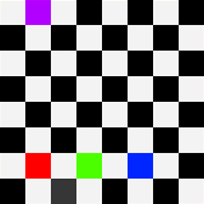
\includegraphics[width=0.25\textwidth]{fig/checker.png}
    \caption{Checker Input Image}
    \label{fig:checker_pattern}
\end{figure}

\begin{figure}
    \centering
    
\includegraphics[width=0.25\textwidth]{fig/random_noise.png}
    \caption{Random Noise Input Image}
    \label{fig:random_noise}
\end{figure}

This section provides a few captures of simulation inputs and outputs in order to show how packets arrive and are processed by the architecture.

In Figure~\ref{fig:input_example} simulated HDMI is shown. When video data enable (write enable) goes high words of data representing PDP packets start to stream in. These are indicated by Packet ID, X start, X end, Y start, Y end, and Packet Data. Each word would be stored in an SCB slot as indicated in the previous section. The final piece of data indicated is a reset packet. Note, that the data prior to Packet ID would be ignored as it does not represent a valid PDP command. It would be discarded by the valid controller.

\begin{figure}
    \centering
    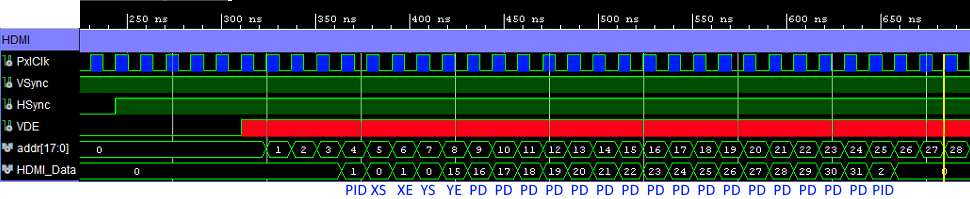
\includegraphics[width=1.0\textwidth]{fig/pdp_input_example.png}
    \caption{PDP Single HDMI Input Example Simulation}
    \label{fig:input_example}
\end{figure}

Figure~\ref{fig:output_example} shows the final output driven to the array. Highlighted in red is data from the write enable packet. Note, all values out are up shifted by 5 bits to be received by the DACs in the system. Additionally, the values are shown in reverse order from the input diagram. For example, 992 corresponds to the value of 31 on the input side. In purple the reset packet is shown with two stages of array writes. In the first stage, load line goes low. In the second stage the load line goes high.

\begin{figure}
    \centering
    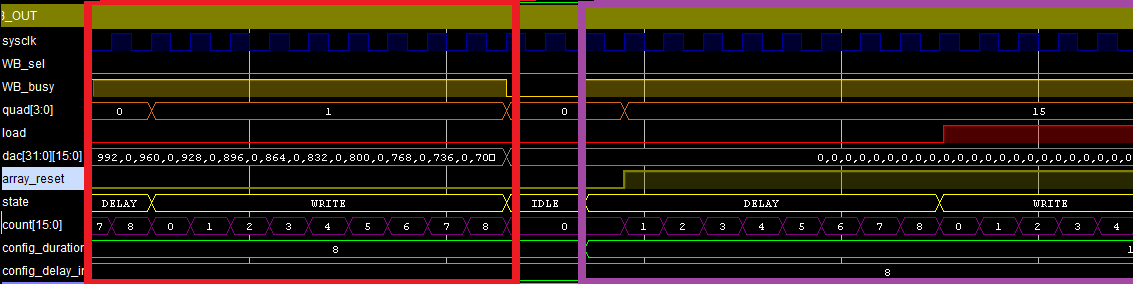
\includegraphics[width=1.0\textwidth]{fig/pdp_output_example.png}
    \caption{PDP Output Example Simulation}
    \label{fig:output_example}
\end{figure}
